\chapter{Write Back}


\begin{figure}
\caption{Write Back}\label{fig:wb}
\begin{center}
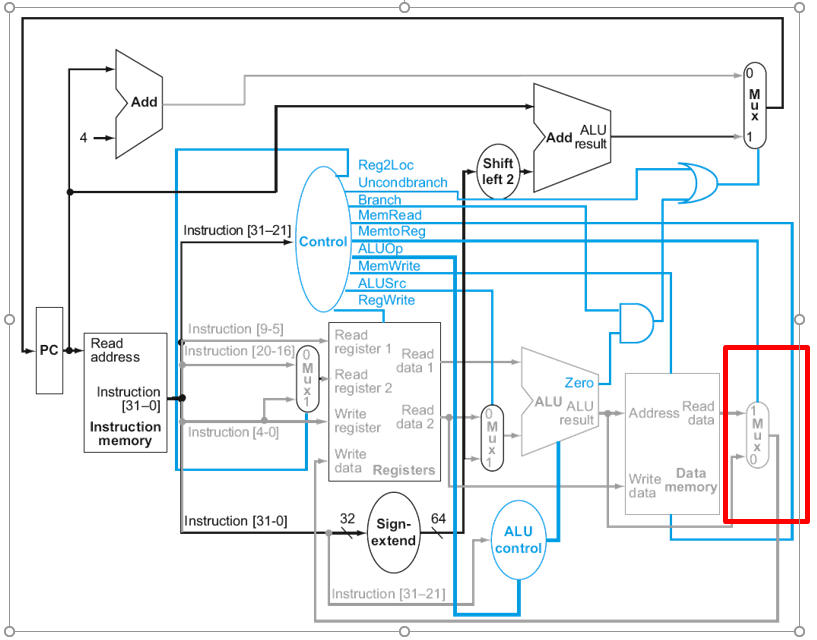
\includegraphics[width=\textwidth]{../images/writeback_stage.png}
\end{center}
\end{figure}

\WrapBarrier

\section{Mux}
This stage consists on only one item, a mux to select between the output of memory and the output of the ALU.  The control is the MemtoReg control line, see Fig~\ref{fig:wb}.  Since the mux has already been tested it does not need a testbench.  The stage thus has only 3 inputs (2 data and 1 control) and one output, the result.

\section{Datapath}
You are ready to assemble the full non-pipelined datapath shown in Fig~\ref{fig:datapath}.  To do this, you will need to combine all 5 stages into datapath.sv.  datapath.sv is a new top-level file, so it is the testbench.  Verify operation of your datapath by running your set of instructions in instrData.data and testing the output.  These instructions are the 10 instructions from the Expected Results Table.  

Now that we have a writeback stage, we do not need to set write\_data in the initial section of datapath.sv.  Rather, you should connect write\_data from the WriteBack stage to the Decode stage.  Because we now have a memory stage, we should no longer need to set pc\_src in the inital section of datapath.sv.  However, our test instructions are not meant to run like a program and would yield strange results.  So for right now, we want to keep pc\_src hard-coded to 0 in datapath.sv.  To do this, we will use a new reg called pc\_src\_tmp and set it to 0.  Then we will use pc\_src\_tmp as the input to the iFetch module.  pc\_src will be a wire that is an output of the iMemory module.  In part 2 of this lab, we will get rid of pc\_src\_tmp and connect pc\_src from iMemory to iFetch.

\begin{figure}
\caption{Full Non-Pipelined Datapath}\label{fig:datapath}
\begin{center}
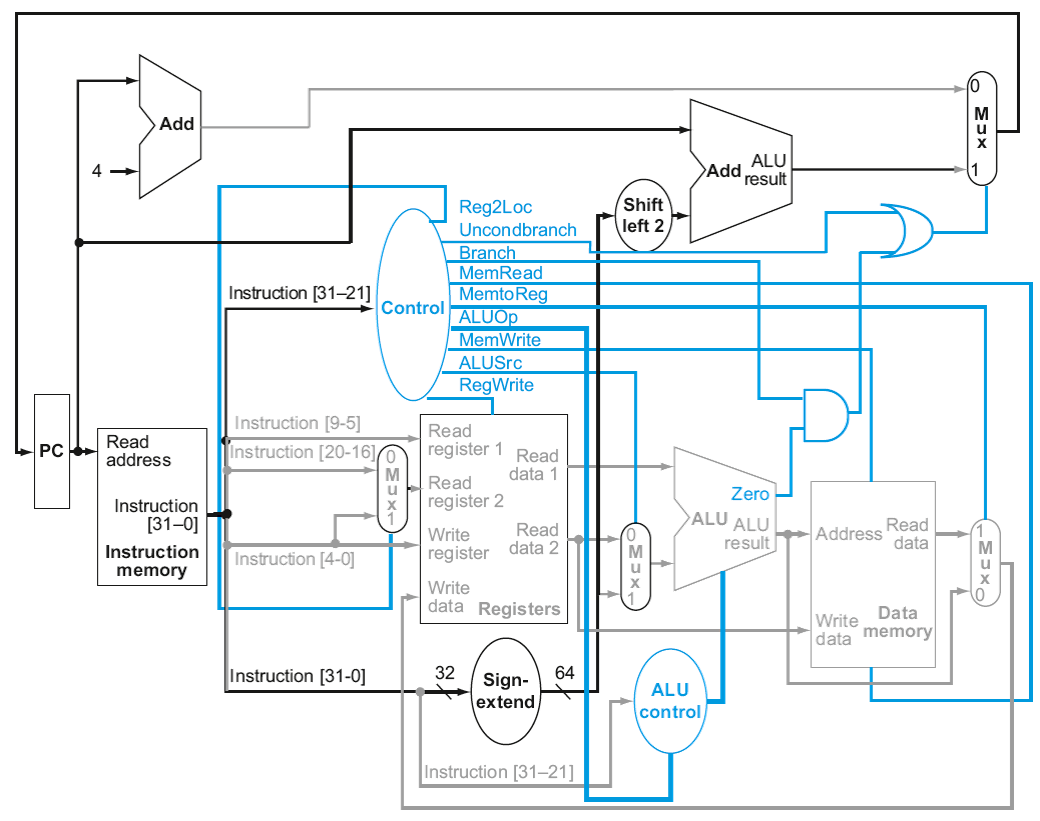
\includegraphics[width=\textwidth]{../images/non_pipelined_datapath.png}
\end{center}
\end{figure}

\section{Your Assignment Part 1}

You are to:
\begin{enumerate}
\item Update your Expected Results Table to include the iWriteBack stage.
\item Create the iWriteback stage consisting of one Mux.
\item Integrate all five stages into the file datapath.sv.
\item Run simulations to verify that your results match your Expected Results table.   
\item There will be one final test to add before we submit it.  However, please save copies of the following:
\begin{enumerate}
	\item A snip of the Simulation Results for datapath.sv.  Please show instructions in hex, opcodes and control signals in binary and everything else in signed decimal.  
	\item Copy and paste the entire log from BEGIN TEST RESULTS to END TEST RESULTS into your file.  The results have gotten too long to use the snipping tool.
\end{enumerate} 
\end{enumerate} 

\section{Division}
To fully verify your LEGv8 processor, we are going to write a program that can divide two numbers, run that program and verify that we get the correct result.  The program that we will run is shown in the file division.c, shown below.  At the top of that file, I've listed some rules about the contents of the regData file and the ramData file.  In previous semesters, I have made students translate this C code into assembly, then translate that assembly into machine code, and put that machine code in instrData.  This semester, to lighten your load, I am providing 2 new files:
\begin{enumerate}
	\item division\_assembly.txt
	\item instrData\_division.data
\end{enumerate}

While I am providing these files, please open the up and analyze the contents.  To utilize these files, you need to copy them into your testfiles directory and update definitions.vh to point to instrData\_division.data.  instrData\_division contains the machine code for the C code listed below.  The assembly translation is also shown below.  Also, you should create a new file called regData\_division.data. You must set all register values in regData\_division.data to 0 except for A22, which should be set to 24.  This value is the base address of the array A.  This is the only non-zero value allowed in regData.  You should also create ramData\_division.  It should have all values set to 0 except for the values of A[0], A[1], A[2], and A[3].  Please set the dividend to 56 and the divisor to 8.  The quotient is initially set to 0.  A[3] is set to 1.  This is necessary because we do not have immediate instructions in our processor.

To verify operation, you should create a final test bench (division.sv) that is the same as datapath.sv except that it allows pc\_src to be set by the iMemory module rather than keeping it hard-coded to 0.  These instructions are meant to run as a program and correct branch decisions are vital to its operation.  The test bench verification is very simple.  It has one test case, which verifies the value that is being stored by the final instruction.  Given that we are calculating 56/8, the result should be 7.  Rather than verifying hundreds of steps along the way (which we've already done), we will very simply check to see if the division works by checking the value of read\_data2 in the final instruction (STUR).  Feel free to modify ramData\_division.data to use a different dividend and divisor...but make sure that they are divisible.  57/8 (or anything like that) will not work properly, as it will never break out of the loop.

\Verilog{C code for doing simple division.}{code:division}{../code/division.c}
\Verilog{Assembly code for doing simple division.}{code:division_assembly}{../code/division_assembly.txt}


\section{Your Assignment Part 2}

You are to:
\begin{enumerate}
	\item Create division.sv.
	\item Run the simulation, analyze the results and verify that the divison works correctly.
	\item Rather than writing a lab report, please produce a landscape mode PDF file called Lab12\_lastname.pdf that includes (in this order):
	\begin{enumerate}
		\item Your name and the lab number.
		\item A snip of the Simulation Results for both the datapath.sv test and division.sv.  Please show instructions in hex, opcodes and control signals in binary and everything else in signed decimal.  
		\item Copy and paste the entire log for both datapath.sv and division.sv from BEGIN TEST RESULTS to END TEST RESULTS into your file.  The results have gotten too long to use the snipping tool.	
	\end{enumerate}
\item Upload Lab12\_lastname.pdf file to Canvas.
\item Zip up your ARM-Lab directory and submit it on Canvas as well.  Please make sure that you give me the ARM-Lab directory rather than the ARM-Project directory.  I do not want the project files in the ARM-Project directory.  Before you submit your zip file, extract the file and make sure that the top-level directory is called ARM-Lab and that the lower level directories like code, manual, etc are directly beneath ARM-Lab in the directory structure.  I will extract your zip file and run your code against my correct testbench to verify that your code and testbench work correctly, and it is critical that everyone's directory structure is consistent.
\end{enumerate} 

CONGRATULATIONS!  YOU'VE JUST BUILT A SIMPLE ARMv8 PROCESSOR!!!!